\documentclass[12pt]{article}

\usepackage{amsmath}
\usepackage{amssymb}
\usepackage{graphicx}
\usepackage{booktabs}
\usepackage{geometry}
\usepackage{hyperref}
\usepackage{cite}
\usepackage{array}
\usepackage{multirow}
\usepackage{setspace}
\usepackage{parskip}
\usepackage{float}
\usepackage{subcaption}
\usepackage{tikz}
\usepackage{pgfplots}
\pgfplotsset{compat=1.18}

\geometry{margin=1in}
\setlength{\parindent}{0pt}
\setlength{\parskip}{6pt}

\hypersetup{
    colorlinks=true,
    linkcolor=black,
    citecolor=black,
    urlcolor=black
}

\title{\textbf{A Transformer-Based Deep Learning Recommender System for Personalized Competitive Programming Problem Selection: Architecture, Training, and Empirical Evaluation}}

\author{
Vinay Kamble\\
\texttt{vinaykamble289@gmail.com}
\and
Shreeya Dhond\\
\texttt{shreeyadhond@gmail.com}
\and
Aisshwarya Gurav\\
\texttt{aisshwaryagurav@gmail.com}
\and
Shrejal Bhosale\\
\texttt{bhosaleshrejal28@gmail.com}
}

\begin{document}

\maketitle

\tableofcontents
\listoffigures
\listoftables

\newpage

\begin{abstract}
We present a self-implemented Transformer-based deep learning recommendation system designed to deliver personalized competitive programming problem suggestions. The system is constructed from foundational PyTorch primitives without reliance on high-level training frameworks, and comprises three principal components: a Problem Encoder based on a Transformer architecture with multi-head self-attention, a User Encoder employing a gated fusion of sequential Transformer processing and skill-profile MLP encoding, and a Multi-Task Recommender Model that simultaneously predicts solve probability, helpfulness, and difficulty match. The model was trained in two stages: contrastive pre-training on 3,433 LeetCode problems across 11 topic clusters, followed by supervised multi-task training on 12,000 synthetic user-problem interaction records. Evaluation results demonstrate that the problem encoder achieves a cluster purity of 99.22\%, indicating highly coherent semantic representations. Ranking performance is strong, with NDCG@10 of 75.48\% and Mean Reciprocal Rank (MRR) of 89.66\%. However, classification accuracy for individual predictions is moderate (solve accuracy: 61.33\%; helpful accuracy: 52.00\%; difficulty accuracy: 36.67\%), and calibration quality is rated poor (solve ECE: 20.96\%; helpful ECE: 15.80\%). Inference throughput reaches 2,155.8 problems per second for batch size 100. The full model occupies 6.10\,MB in FP32 precision with 1,600,389 total parameters, making it suitable for resource-constrained deployment. Observed performance gaps, calibration limitations, and directions for improvement are discussed.
\end{abstract}

\newpage

% ------------------------------------------------------------------
\section{Introduction}
% ------------------------------------------------------------------

Selecting an appropriate practice problem is a non-trivial challenge for learners engaged in competitive programming. Problems vary along multiple dimensions---difficulty, topic coverage, algorithmic requirement, and contextual fit for the individual---such that generic curated lists are insufficient for personalized learning. Rule-based systems, while efficient and interpretable, rely on hand-crafted heuristics and fail to capture the nuanced semantic relationships between problem content and user skill trajectories.

Recent advances in deep learning, and specifically Transformer architectures \cite{vaswani2017attention}, offer a principled framework for learning rich representations of both problem content and user behavior. Multi-task learning enables joint optimization over complementary signals such as solve probability, perceived helpfulness, and difficulty appropriateness \cite{kendall2018multitask}. Contrastive pre-training has demonstrated strong performance in learning semantically organized embedding spaces \cite{chen2020simclr}, and attention-based models have shown utility in sequential knowledge tracing settings \cite{pandey2019sakt,ghosh2020akt}.

This paper presents a complete empirical account of a self-implemented system applying these techniques to the domain of competitive programming problem recommendation. The primary contributions documented herein are:

\begin{itemize}
    \item A Transformer-based Problem Encoder pre-trained via contrastive learning (InfoNCE) on a corpus of 3,433 LeetCode problems grouped into 11 topic clusters.
    \item A dual-mode User Encoder with gated fusion of sequential Transformer processing and a skill-profile MLP branch.
    \item A Multi-Task Recommender Model producing three simultaneous outputs: solve probability, helpfulness probability, and difficulty match classification.
    \item Comprehensive empirical evaluation including encoder quality, classification performance, ranking metrics, calibration analysis, inference latency benchmarking, model size characterization, and attention quality assessment.
\end{itemize}

% ------------------------------------------------------------------
\section{Related Work}
% ------------------------------------------------------------------

\subsection{Transformer Architecture and Representation Learning}

The foundational Transformer architecture introduced by Vaswani et al.\ \cite{vaswani2017attention} underlies the Problem Encoder and User Encoder employed in this work. Scaled dot-product attention and multi-head attention enable the model to capture both local and long-range dependencies in token sequences in parallel. The BERT model \cite{devlin2019bert} demonstrated the utility of bidirectional Transformer encoders with special classification tokens ([CLS]) for fixed-length representation extraction, a design pattern directly adopted in this system's Problem Encoder.

\subsection{Knowledge Tracing}

The Self-Attentive Knowledge Tracing (SAKT) model \cite{pandey2019sakt} replaces recurrent architectures with attention mechanisms to model student knowledge states from interaction sequences, yielding improved interpretability and performance over LSTM-based approaches. The Attentive Knowledge Tracing (AKT) model \cite{ghosh2020akt} further introduces context-awareness and attention weighting to capture evolving student proficiency. Both approaches inform the sequential user modeling component of this system.

\subsection{Neural Recommender Systems}

Neural Collaborative Filtering \cite{he2017ncf} established the use of deep neural networks for collaborative filtering, replacing matrix factorization with multi-layer perceptrons to model user-item interactions. The survey by Zhang et al.\ \cite{zhang2019dlrecsys} provides a comprehensive treatment of deep learning-based recommender system architectures, motivating the design of the multi-task interaction layer employed herein.

\subsection{Learning Analytics and Student Modeling}

Learning Factors Analysis \cite{cen2006lfa} provides an alternative to Bayesian Knowledge Tracing for modeling learning curves, offering a comparative basis for approaches to student skill modeling. Whitehill et al.\ \cite{whitehill2017mooc} demonstrate performance prediction in MOOCs using behavioral data, grounding the real-world applicability of student modeling systems.

\subsection{Calibration}

Guo et al.\ \cite{guo2017calibration} characterize the calibration properties of modern neural networks and introduce temperature scaling as a post-hoc calibration technique. Their findings are directly relevant to the calibration analysis of this system, where Expected Calibration Error (ECE) is used as the primary calibration metric.

\subsection{Ranking and Evaluation}

Liu \cite{liu2009l2r} provides the theoretical foundation for learning-to-rank, underpinning the use of NDCG and MRR as ranking evaluation metrics in this work.

% ------------------------------------------------------------------
\section{Methodology}
% ------------------------------------------------------------------

\subsection{System Overview}

The system operates as a three-stage pipeline, as illustrated in Figure~\ref{fig:architecture}. First, the Problem Encoder transforms raw problem metadata (title, description, tags, and difficulty) into a 64-dimensional L2-normalized embedding. Second, the User Encoder ingests the user's interaction history and skill profile to produce a 64-dimensional L2-normalized user embedding. Third, the Recommender Model combines both embeddings through a structured interaction layer and three residual blocks, producing multi-task prediction outputs.

\begin{figure}[H]
\centering
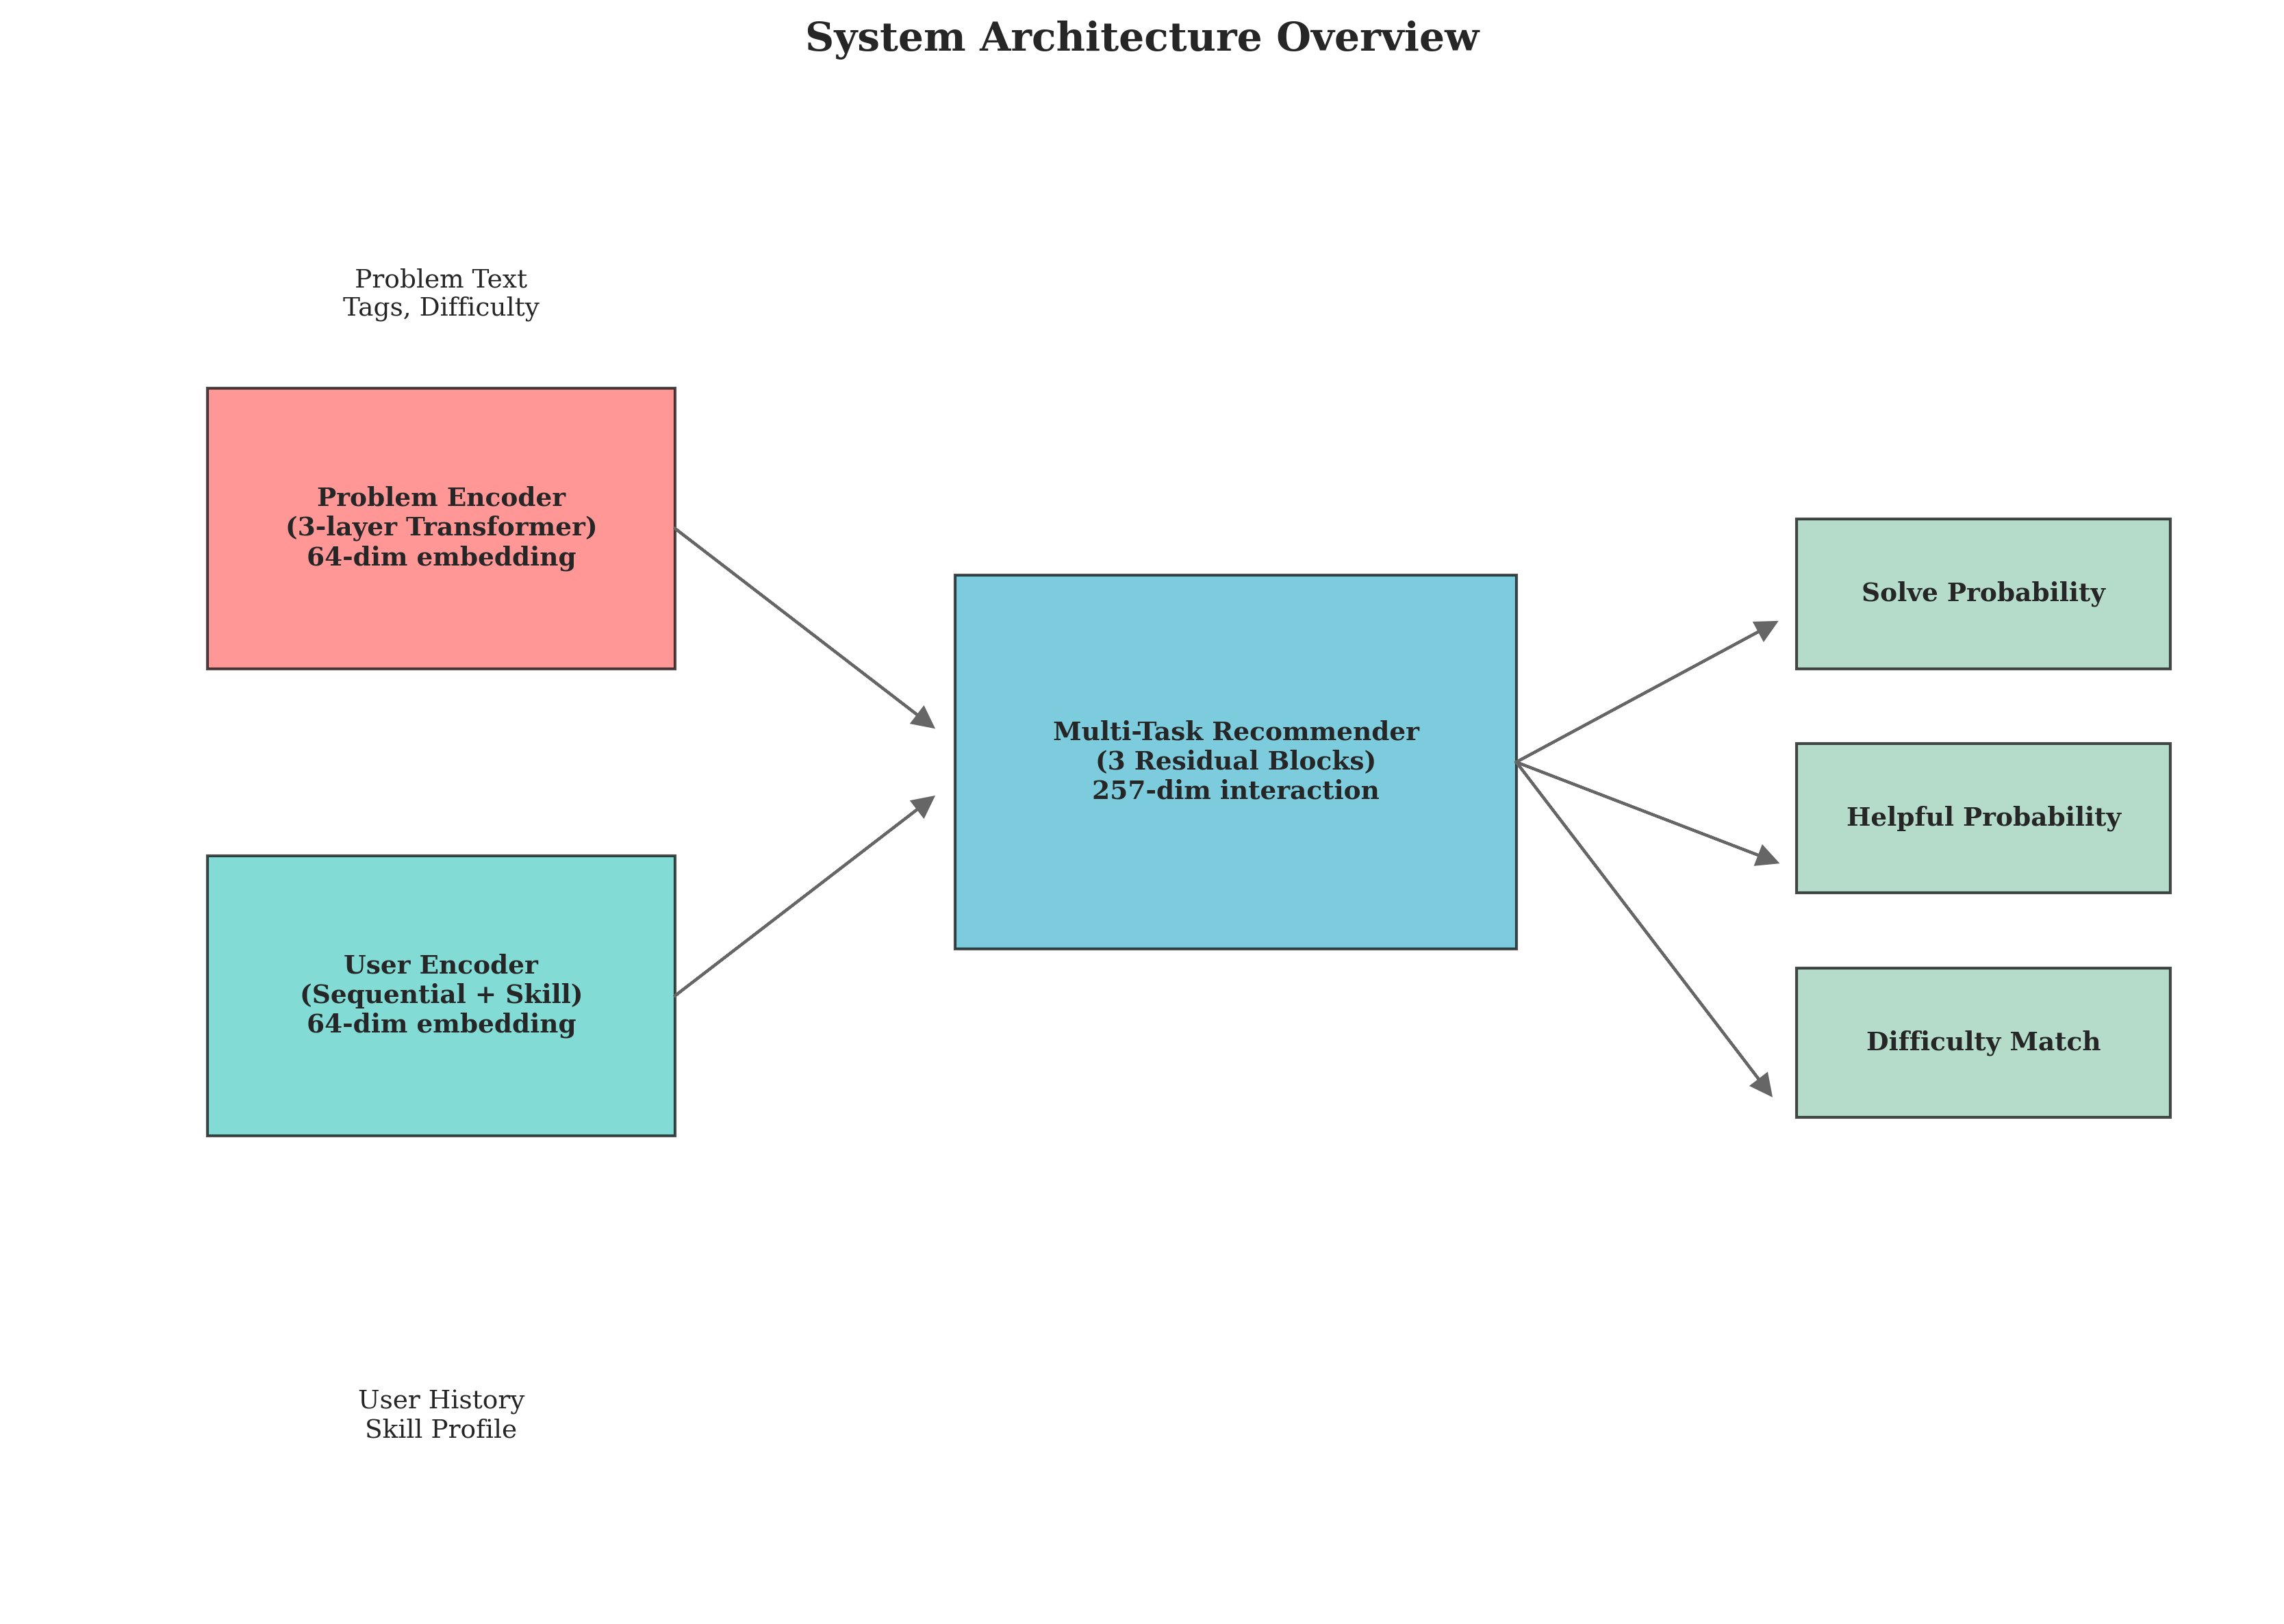
\includegraphics[width=0.9\textwidth]{architecture_diagram.png}
\caption{System Architecture Overview. The system comprises three main components: a Transformer-based Problem Encoder, a dual-mode User Encoder with gated fusion, and a Multi-Task Recommender Model producing three simultaneous outputs.}
\label{fig:architecture}
\end{figure}

\subsection{Problem Encoder}

\subsubsection{Architecture}

The Problem Encoder is a Transformer encoder comprising 3 layers, 4 attention heads, model dimension $d_{\text{model}} = 128$, feed-forward inner dimension $d_{\text{ff}} = 512$, maximum sequence length $L_{\max} = 64$ tokens, vocabulary size $V = 2{,}329$, and dropout rate $p = 0.1$.

A special [CLS] token is prepended to each tokenized problem sequence. After three Transformer encoder layers, the [CLS] token representation is projected from 128 to 64 dimensions via a learned MLP and L2-normalized to produce the problem embedding.

\subsubsection{Input Construction}

Token embeddings $\mathbf{E} \in \mathbb{R}^{V \times d_{\text{model}}}$ are scaled by $\sqrt{d_{\text{model}}}$ and summed with sinusoidal positional encodings:
\begin{align}
\text{PE}(\text{pos}, 2i) &= \sin\!\left(\frac{\text{pos}}{10000^{2i/d_{\text{model}}}}\right), \\
\text{PE}(\text{pos}, 2i+1) &= \cos\!\left(\frac{\text{pos}}{10000^{2i/d_{\text{model}}}}\right).
\end{align}
Topic tags and difficulty level are injected at the [CLS] position via learned embeddings:
\begin{equation}
\mathbf{X}[0, :] \mathrel{+}= \text{MLP}\!\left([\bar{\mathbf{e}}_{\text{topic}};\, \mathbf{e}_{\text{difficulty}}]\right),
\end{equation}
where $\bar{\mathbf{e}}_{\text{topic}}$ is the mean of topic embeddings and $\mathbf{e}_{\text{difficulty}}$ is a learned difficulty embedding.

\subsubsection{Transformer Encoder Layer}

Each of the three encoder layers applies Pre-Layer Normalization (Pre-LN) before each sub-layer. Multi-head self-attention is computed as:
\begin{equation}
\text{MultiHead}(\mathbf{Q}, \mathbf{K}, \mathbf{V}) = \text{Concat}(\text{head}_1, \ldots, \text{head}_h)\,\mathbf{W}^O,
\end{equation}
where each head is:
\begin{equation}
\text{head}_i = \text{Attention}(\mathbf{Q}\mathbf{W}_i^Q,\, \mathbf{K}\mathbf{W}_i^K,\, \mathbf{V}\mathbf{W}_i^V) = \text{softmax}\!\left(\frac{\mathbf{Q}\mathbf{K}^\top}{\sqrt{d_k}}\right)\mathbf{V},
\end{equation}
with $d_k = d_{\text{model}} / h = 32$ for $h = 4$ heads. The feed-forward sub-layer applies:
\begin{equation}
\text{FFN}(\mathbf{x}) = \text{GELU}(\mathbf{x}\mathbf{W}_1 + \mathbf{b}_1)\mathbf{W}_2 + \mathbf{b}_2,
\end{equation}
where $\mathbf{W}_1 \in \mathbb{R}^{d_{\text{model}} \times d_{\text{ff}}}$ and $\mathbf{W}_2 \in \mathbb{R}^{d_{\text{ff}} \times d_{\text{model}}}$. Residual connections are applied after each sub-layer.

\subsubsection{Contrastive Pre-training}

The Problem Encoder is pre-trained using the InfoNCE (NT-Xent) contrastive loss at temperature $\tau = 0.2$:
\begin{equation}
\mathcal{L}_{\text{contrastive}} = -\log\frac{\exp(\text{sim}(\mathbf{z}_i, \mathbf{z}_j) / \tau)}{\sum_{k} \exp(\text{sim}(\mathbf{z}_i, \mathbf{z}_k) / \tau)},
\end{equation}
where $\text{sim}(\mathbf{z}_i, \mathbf{z}_j) = \mathbf{z}_i \cdot \mathbf{z}_j$ (cosine similarity over L2-normalized embeddings), $j$ is a positive sample from the same topic cluster as $i$, and $k$ ranges over all other samples in the batch (negatives).

\subsection{User Encoder}

The User Encoder combines two parallel encoding modes via a learned gated fusion mechanism.

\subsubsection{Mode A: Sequential Encoder}

A 2-layer Transformer processes the chronologically ordered sequence of solved problem embeddings prepended by a learned [USER] token. Learnable positional encodings capture temporal order, and difficulty embeddings are injected at each position:
\begin{equation}
\mathbf{S} = [\mathbf{u}_{\text{USER}};\, \mathbf{h}_1 + \mathbf{p}_1 + \mathbf{d}_1;\, \ldots;\, \mathbf{h}_n + \mathbf{p}_n + \mathbf{d}_n],
\end{equation}
where $\mathbf{h}_i$ is the pre-computed problem embedding, $\mathbf{p}_i$ is the learnable positional embedding, and $\mathbf{d}_i$ is the difficulty embedding at position $i$. The [USER] token representation at position 0 after Transformer processing constitutes the sequential embedding $\mathbf{e}_{\text{seq}}$.

\subsubsection{Mode B: Skill Profile Encoder}

A 44-dimensional skill vector $\mathbf{s} \in \mathbb{R}^{44}$, comprising topic occurrence counts (40 dimensions), difficulty distribution ratios (3 dimensions), and current problem-solving streak (1 dimension), is encoded by a two-layer MLP with GELU activation:
\begin{equation}
\mathbf{e}_{\text{skill}} = \text{LayerNorm}(\text{Linear}_2(\text{Dropout}(\text{GELU}(\text{Linear}_1(\mathbf{s}))))),
\end{equation}
where $\text{Linear}_1: 44 \to 128$ and $\text{Linear}_2: 128 \to 64$.

\subsubsection{Gated Fusion}

The two representations are fused via a learned gate:
\begin{align}
\mathbf{g} &= \sigma\!\left(\mathbf{W}_{\text{gate}}\,[\mathbf{e}_{\text{seq}};\, \mathbf{e}_{\text{skill}}] + \mathbf{b}_{\text{gate}}\right), \\
\mathbf{e}_{\text{user}} &= \mathbf{g} \odot \mathbf{e}_{\text{seq}} + (1 - \mathbf{g}) \odot \mathbf{e}_{\text{skill}},
\end{align}
where $\mathbf{W}_{\text{gate}} \in \mathbb{R}^{64 \times 128}$ and $\sigma$ is the sigmoid function. The final user embedding is L2-normalized.

\subsection{Recommender Model}

\subsubsection{Interaction Layer}

The interaction representation is constructed from the L2-normalized user embedding $\mathbf{u} \in \mathbb{R}^{64}$ and problem embedding $\mathbf{p} \in \mathbb{R}^{64}$:
\begin{equation}
\mathbf{i} = [\mathbf{u};\, \mathbf{p};\, \mathbf{u} \odot \mathbf{p};\, |\mathbf{u} - \mathbf{p}|;\, \mathbf{u} \cdot \mathbf{p}] \in \mathbb{R}^{4 \times 64 + 1 = 257}.
\end{equation}

\subsubsection{Residual MLP}

The interaction vector is projected to the hidden dimension $d_{\text{hidden}} = 256$ and then processed by 3 residual blocks:
\begin{equation}
\mathbf{h}^{(l)} = \text{LayerNorm}\!\left(\mathbf{h}^{(l-1)} + \text{Dropout}(\text{Linear}_2(\text{GELU}(\text{Linear}_1(\mathbf{h}^{(l-1)}))))\right),
\end{equation}
where both linear layers map $256 \to 256$.

\subsubsection{Multi-Task Output Heads}

Three output heads operate on the shared representation $\mathbf{h}^{(3)}$:

\begin{align}
p_{\text{solve}} &= \sigma(\mathbf{w}_{\text{solve}}^\top \mathbf{h}^{(3)} + b_{\text{solve}}), \\
p_{\text{helpful}} &= \sigma(\mathbf{w}_{\text{helpful}}^\top \mathbf{h}^{(3)} + b_{\text{helpful}}), \\
\mathbf{p}_{\text{diff}} &= \text{softmax}(\mathbf{W}_{\text{diff}}\,\mathbf{h}^{(3)} + \mathbf{b}_{\text{diff}}) \in \mathbb{R}^3.
\end{align}

The difficulty classes are indexed as: 0 = too easy, 1 = just right, 2 = too hard.

\subsubsection{Multi-Task Loss}

The combined training loss is a weighted sum:
\begin{equation}
\mathcal{L} = 0.4\,\mathcal{L}_{\text{solve}} + 0.3\,\mathcal{L}_{\text{helpful}} + 0.3\,\mathcal{L}_{\text{difficulty}},
\end{equation}
where $\mathcal{L}_{\text{solve}}$ and $\mathcal{L}_{\text{helpful}}$ are binary cross-entropy losses and $\mathcal{L}_{\text{difficulty}}$ is a categorical cross-entropy loss.

\subsection{Optimizer and Learning Rate Schedule}

Optimization uses a self-implemented AdamW optimizer with $\alpha = 3 \times 10^{-4}$, $\beta_1 = 0.9$, $\beta_2 = 0.999$, $\varepsilon = 10^{-8}$, and weight decay $\lambda = 0.01$. Gradient clipping is applied at $\|\nabla\|_{\max} = 1.0$. The learning rate schedule applies warmup over 10\% of training steps, followed by cosine annealing:
\begin{equation}
\alpha_t = \alpha_{\min} + \tfrac{1}{2}(\alpha_{\max} - \alpha_{\min})\left(1 + \cos\!\left(\pi \cdot \frac{t - t_{\text{warmup}}}{T - t_{\text{warmup}}}\right)\right),
\end{equation}
where $\alpha_{\max} = 3 \times 10^{-4}$, $\alpha_{\min} = 3 \times 10^{-6}$, and $T$ is the total number of training steps.

\subsection{Exploration Strategies}

At inference time, two exploration strategies are supported. Under epsilon-greedy ($\varepsilon = 0.15$), a uniformly random problem is selected with probability $\varepsilon$; otherwise the highest-scoring problem is returned. Under Upper Confidence Bound (UCB1), recommendations are scored as:
\begin{equation}
\text{UCB}_i = \text{score}_i + c\sqrt{\frac{\ln N}{n_i}},
\end{equation}
where $N$ is the total number of recommendations made, $n_i$ is the number of times problem $i$ has been recommended, and $c = 1.0$ is the exploration constant.

% ------------------------------------------------------------------
\section{Experimental Setup}
% ------------------------------------------------------------------

\subsection{Dataset}

The problem dataset comprises 3,851 total problems sourced from a LeetCode Questions XLSX file, of which 3,433 are algorithmically categorized and used for encoder training. The difficulty distribution is approximately 35\% Easy, 47\% Medium, and 18\% Hard. Problems span over 40 distinct topic tags and are grouped into 11 topic clusters for contrastive pre-training.

For recommendation model training, 12,000 synthetic user-problem interaction records were generated, representing 300 synthetic users (100 each of Beginner, Intermediate, and Advanced profiles) with 40 interactions per user. Ground-truth labels cover solve outcome, helpfulness, and difficulty perception (balanced across three classes). No real user interaction data was employed in any stage of the training reported herein.

\subsection{Training Configuration}

\textbf{Stage 1 (Pre-training):} 15 epochs on the 3,433-problem corpus; batch size 64; AdamW optimizer; InfoNCE contrastive loss at $\tau = 0.2$. Best validation checkpoint at epoch 8 (validation loss: 2.70).

\textbf{Stage 2 (Recommendation Model):} 30 epochs on 12,000 synthetic interaction records; batch size 64; AdamW; weighted multi-task loss. Best validation checkpoint selected at epoch 5 (validation loss: 0.76).

\subsection{Evaluation Protocol}

The evaluation framework encompasses five metric categories drawn from the evaluation report:

\begin{itemize}
    \item \textbf{Encoder Quality:} Nearest-neighbor cluster purity, embedding alignment loss, uniformity loss, contrastive loss, and embedding norm statistics ($n = 512$ samples).
    \item \textbf{Classification Performance:} Accuracy, AUC, F1, precision, recall, and Brier Score for solve and helpful predictions; accuracy and per-class accuracy for difficulty prediction ($n_{\text{val}} = 300$ samples).
    \item \textbf{Ranking Performance:} NDCG@$k$, Precision@$k$, Recall@$k$ for $k \in \{5, 10, 20\}$, and MRR, evaluated over 29 sessions.
    \item \textbf{Calibration:} Expected Calibration Error (ECE) for solve and helpful tasks, computed over 10 equal-width confidence bins.
    \item \textbf{Inference Latency:} Per-component and total latency at batch sizes 1, 10, 50, 100, and 200; throughput in problems per second.
\end{itemize}

% ------------------------------------------------------------------
\section{Results}
% ------------------------------------------------------------------

This section presents comprehensive empirical results across five evaluation categories: encoder quality, classification performance, ranking metrics, calibration analysis, and computational efficiency. Figure~\ref{fig:performance_overview} provides a high-level overview of the key performance metrics.

\begin{figure}[H]
\centering
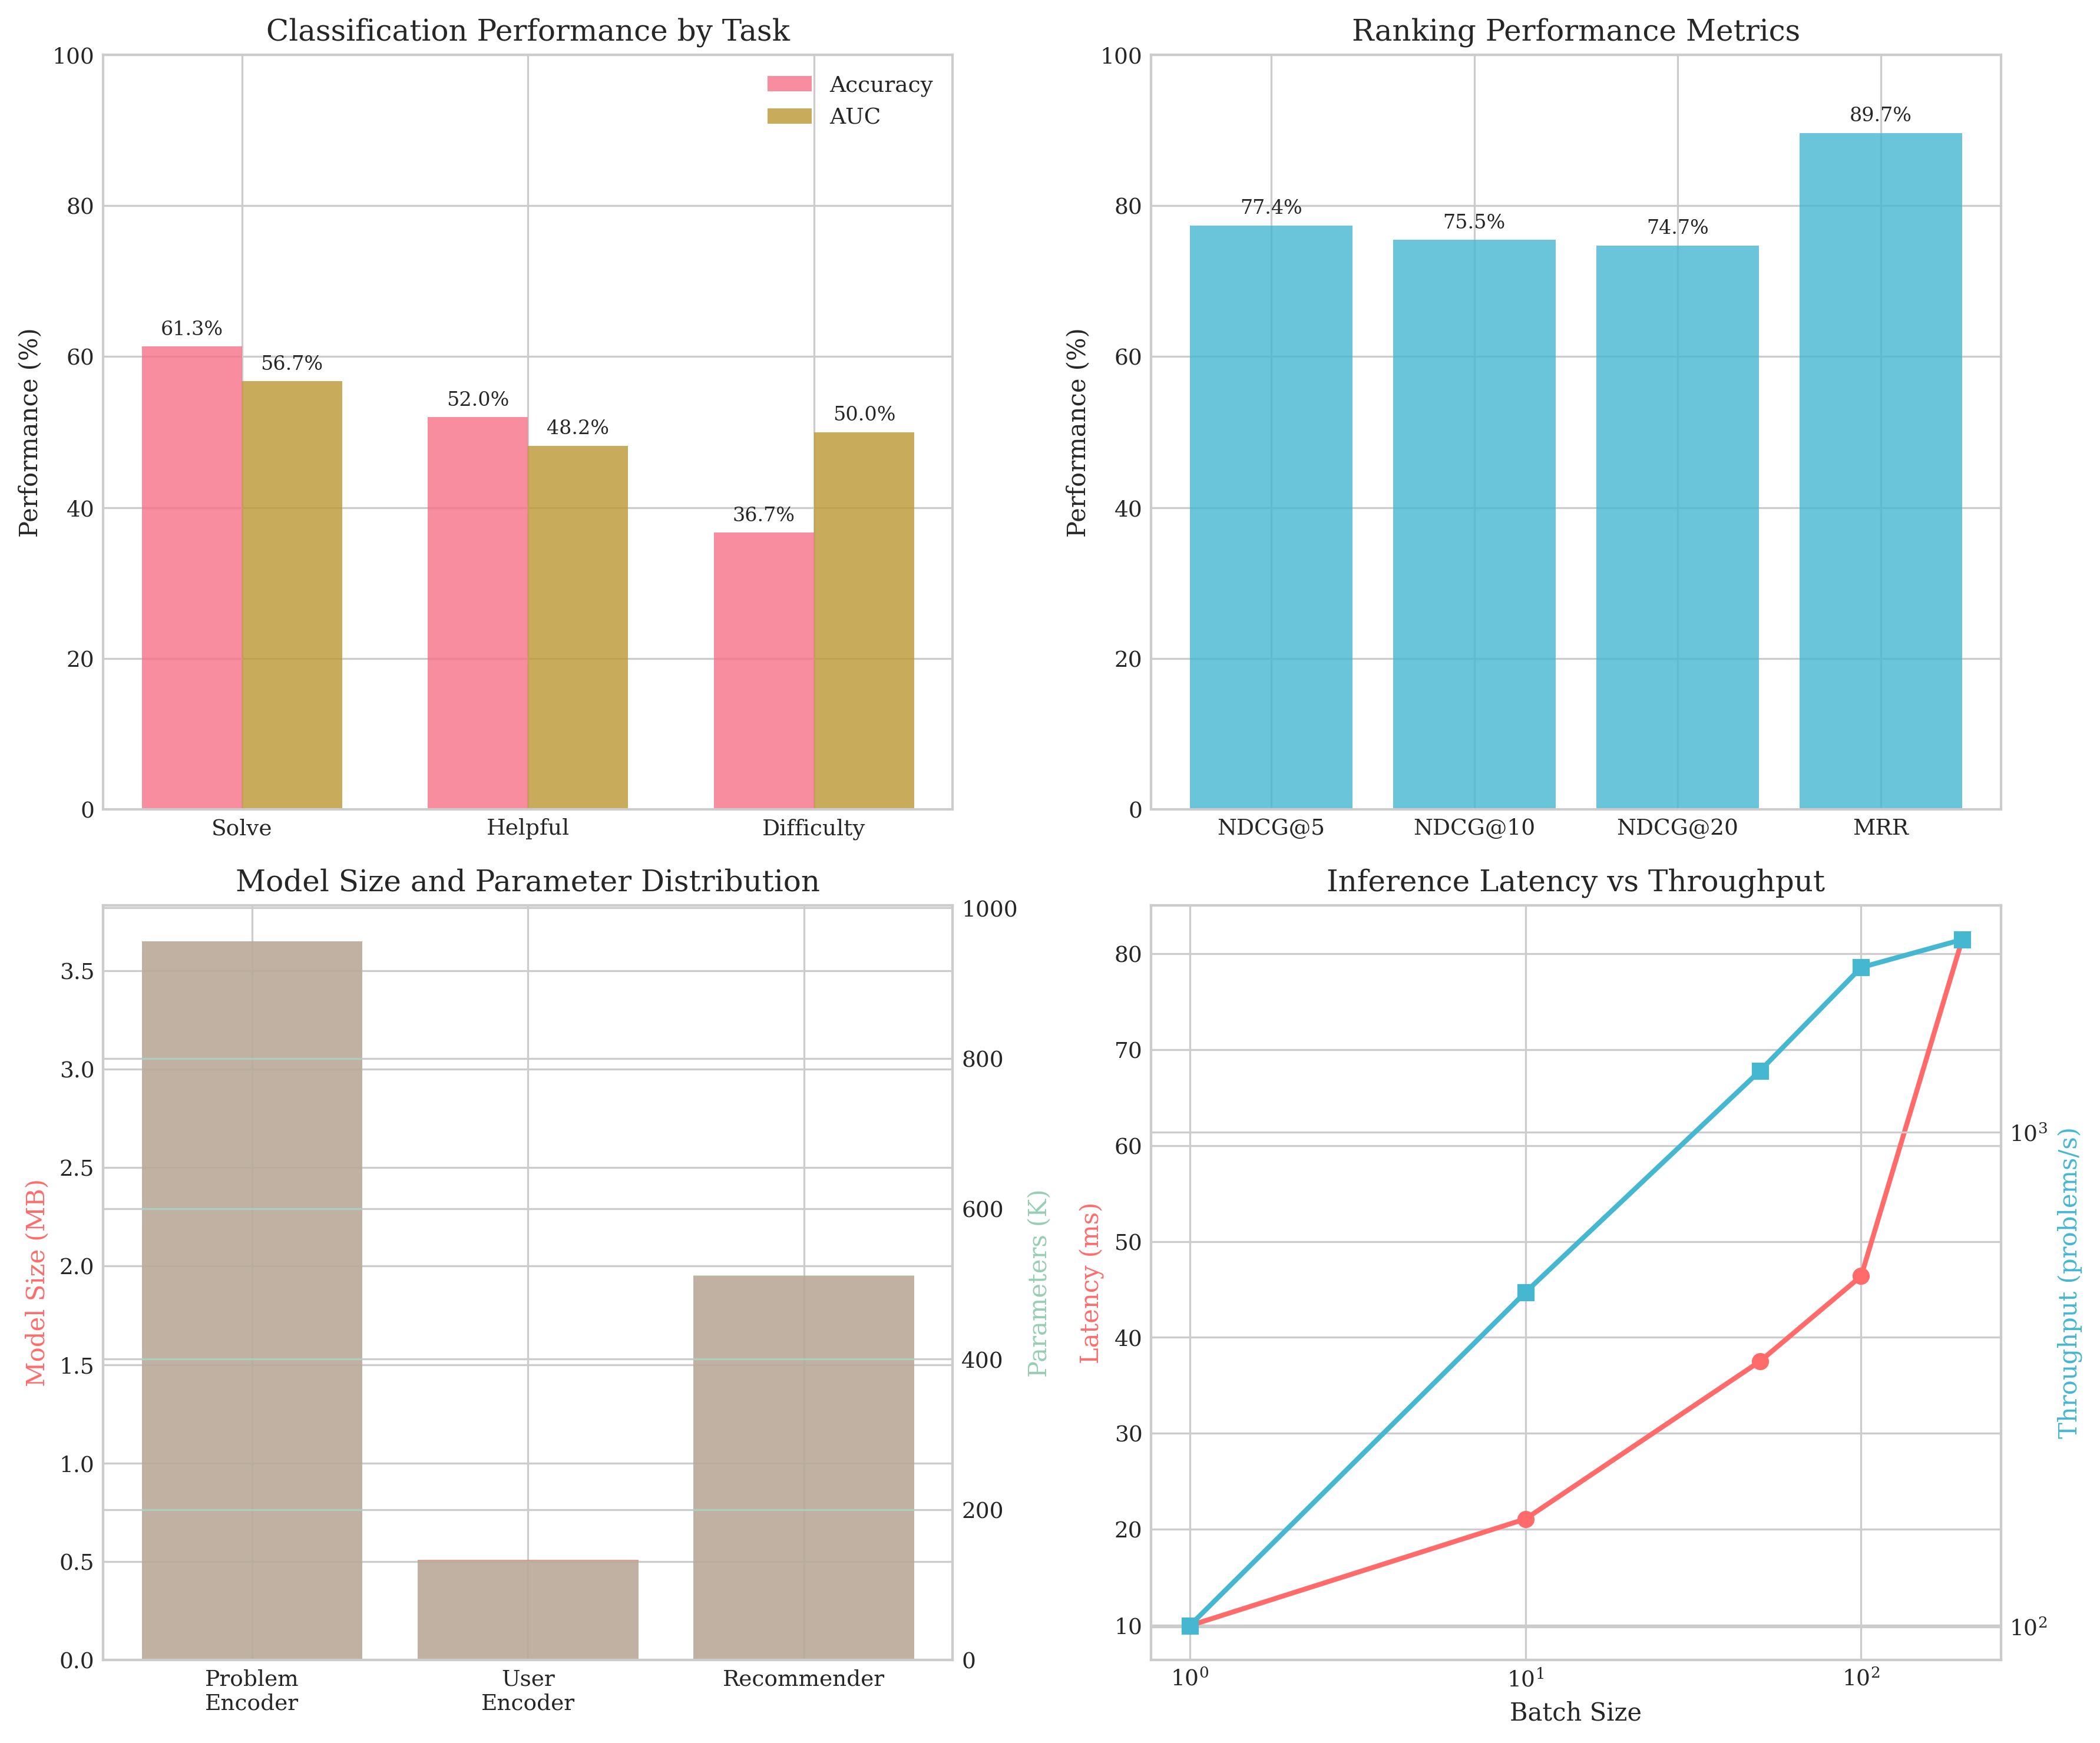
\includegraphics[width=\textwidth]{performance_metrics.png}
\caption{Comprehensive Performance Overview. (Top Left) Classification accuracy and AUC by task. (Top Right) Ranking performance metrics showing strong NDCG and MRR scores. (Bottom Left) Model size distribution across components. (Bottom Right) Inference latency and throughput scaling with batch size.}
\label{fig:performance_overview}
\end{figure}

\subsection{Encoder Quality}

Table~\ref{tab:encoder} reports problem encoder quality metrics evaluated on 512 samples. Figure~\ref{fig:encoder_quality} provides detailed visualizations of encoder performance across multiple dimensions.

\begin{figure}[H]
\centering
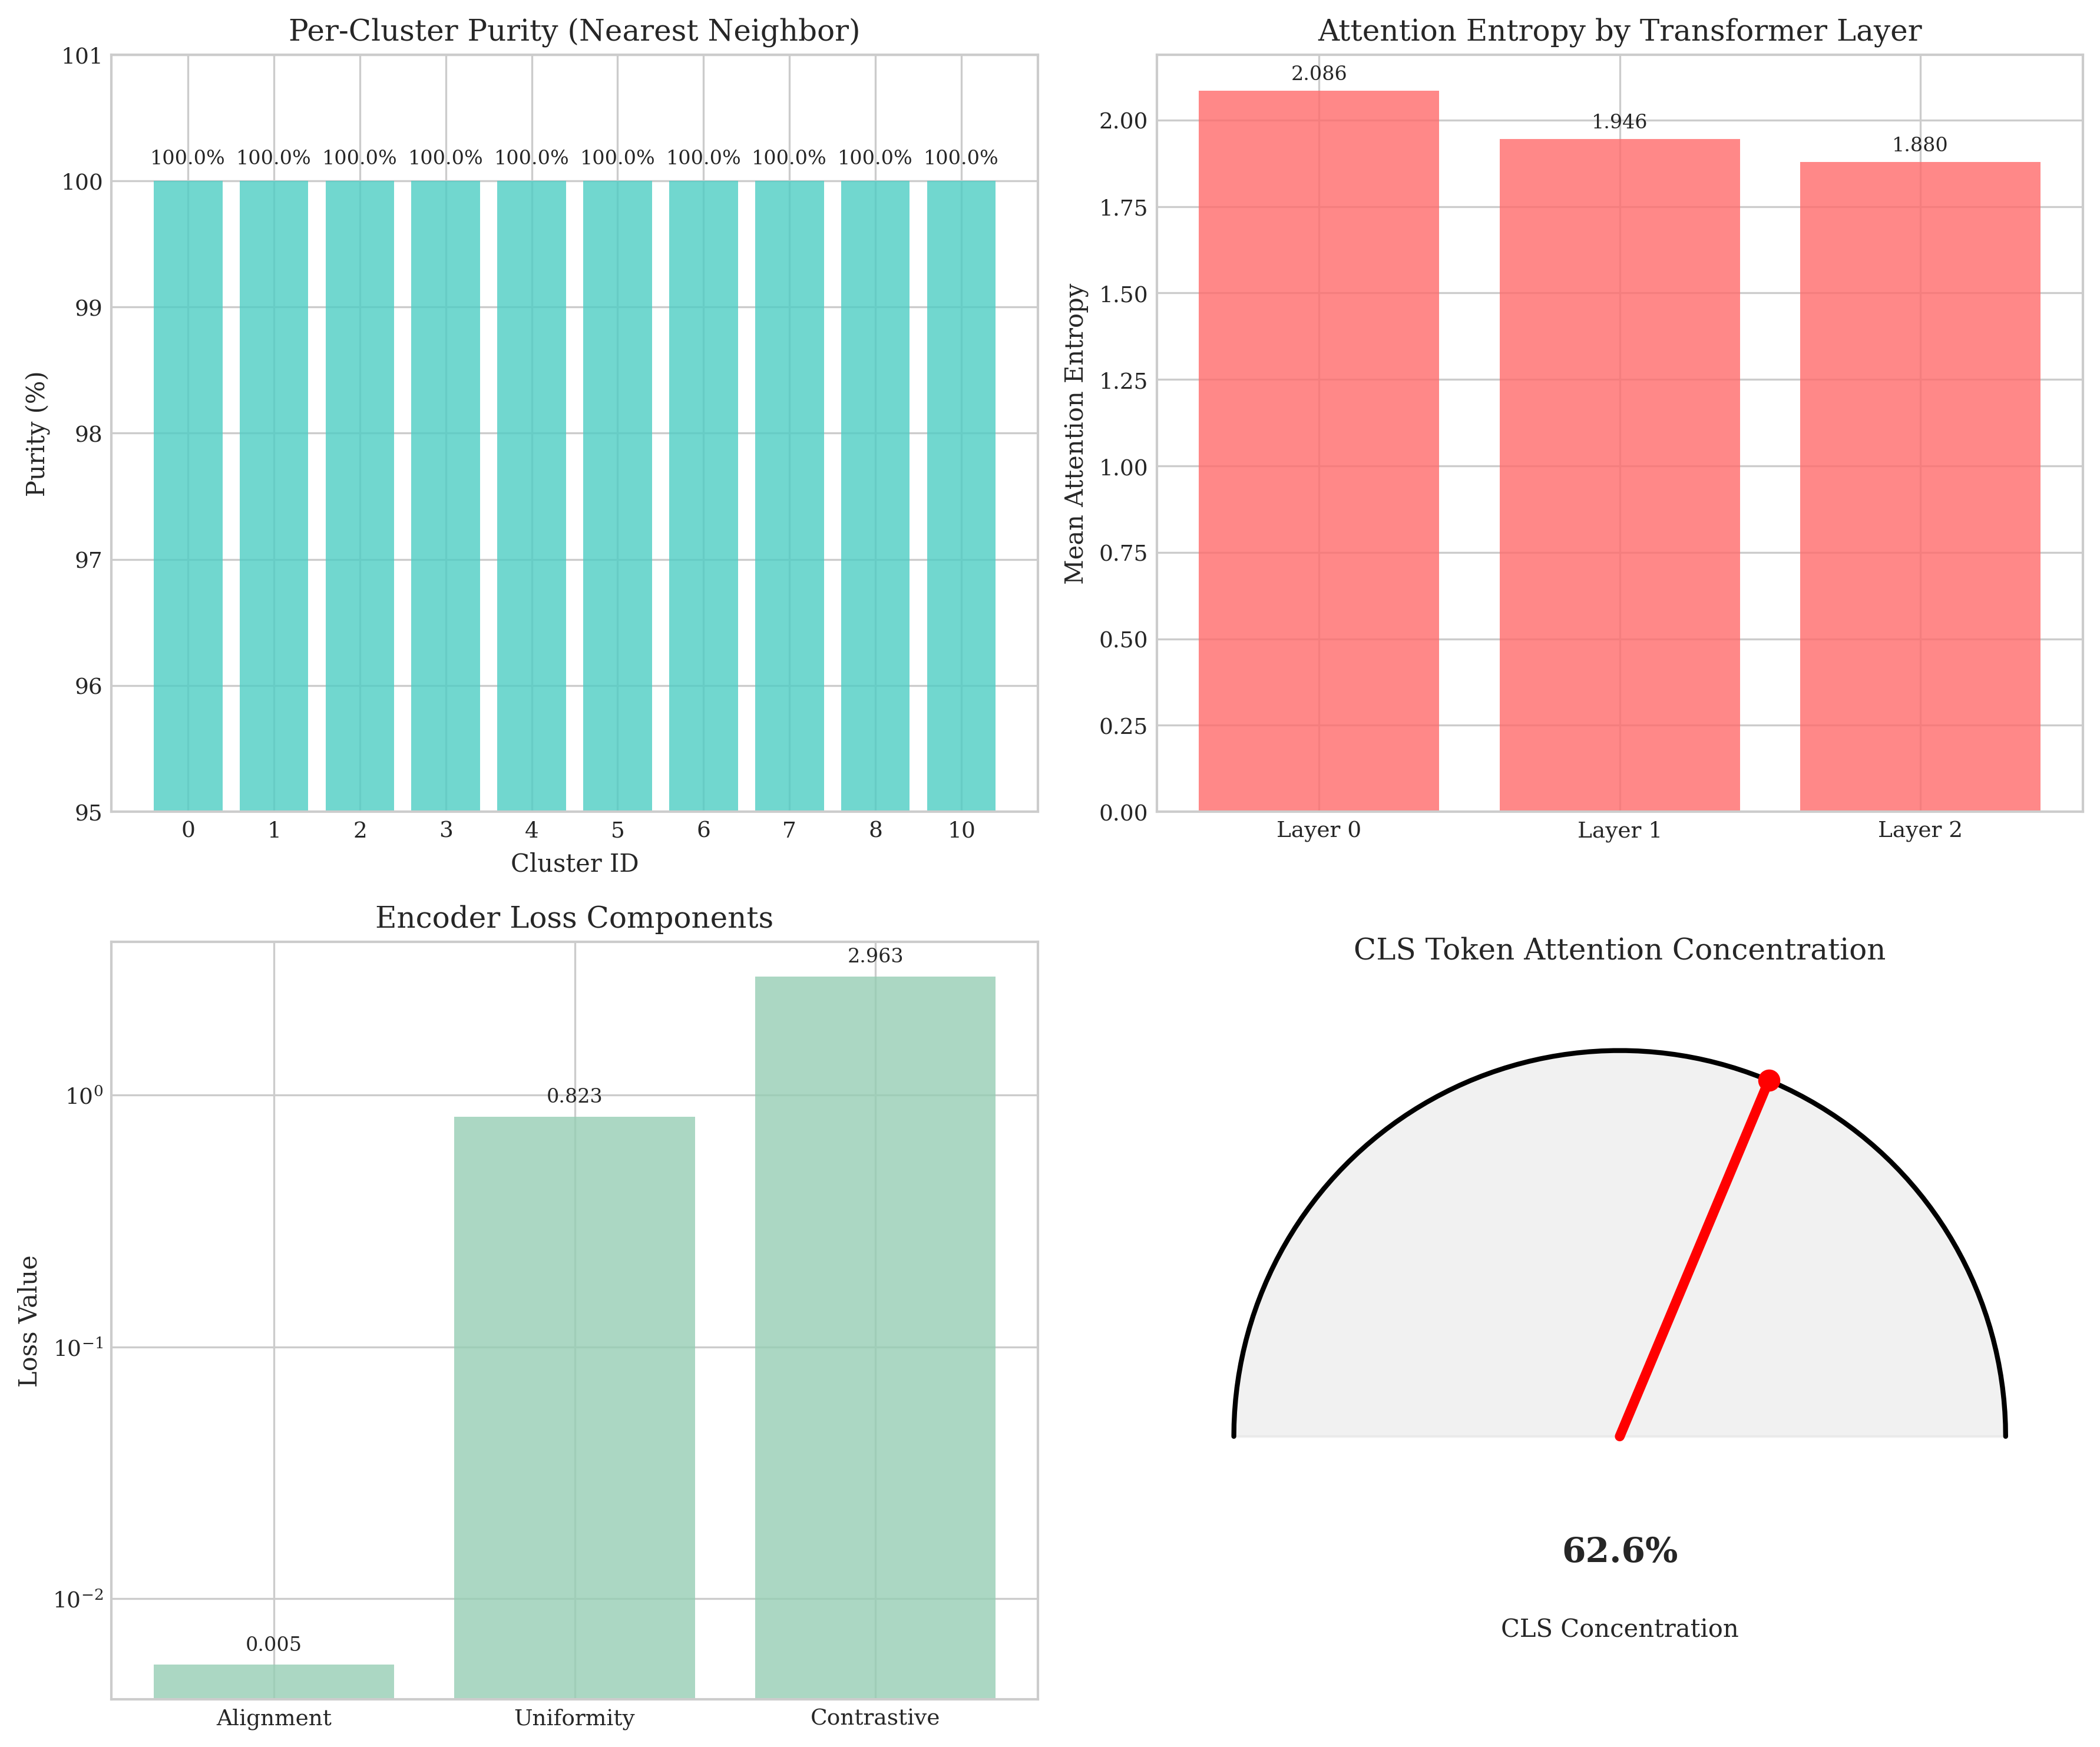
\includegraphics[width=\textwidth]{encoder_quality.png}
\caption{Problem Encoder Quality Analysis. (Top Left) Per-cluster purity showing near-perfect semantic organization. (Top Right) Attention entropy decreasing across Transformer layers. (Bottom Left) Loss component magnitudes on logarithmic scale. (Bottom Right) CLS token attention concentration gauge.}
\label{fig:encoder_quality}
\end{figure}

\begin{table}[H]
\centering
\caption{Problem Encoder Quality Metrics ($n = 512$ samples).}
\label{tab:encoder}
\begin{tabular}{lc}
\toprule
\textbf{Metric} & \textbf{Value} \\
\midrule
Cluster Purity (Nearest Neighbour) & 99.22\% \\
Alignment Loss & 0.0055 \\
Uniformity Loss & $-$0.8228 \\
Contrastive Loss & 2.9626 \\
Mean Embedding Norm & 1.0 (std $\approx 3.8 \times 10^{-8}$) \\
\bottomrule
\end{tabular}
\end{table}

Per-cluster purity of 100\% is achieved for 10 of the 11 evaluated clusters (clusters 0 through 8 and cluster 10). Per-cluster data for cluster 9 is absent from the evaluation report.

\subsection{Attention Quality}

Table~\ref{tab:attention} reports attention entropy and CLS concentration metrics evaluated on 224 samples.

\begin{table}[H]
\centering
\caption{Attention Quality Metrics ($n = 224$ samples).}
\label{tab:attention}
\begin{tabular}{lc}
\toprule
\textbf{Metric} & \textbf{Value} \\
\midrule
Layer 0 Mean Entropy & 2.0856 \\
Layer 1 Mean Entropy & 1.9456 \\
Layer 2 Mean Entropy & 1.8796 \\
CLS Concentration Mean & 62.63\% \\
\bottomrule
\end{tabular}
\end{table}

\subsection{Classification Performance}

Table~\ref{tab:classification} presents classification metrics evaluated on 300 validation samples.

\begin{table}[H]
\centering
\caption{Classification Performance on the 300-Sample Validation Set.}
\label{tab:classification}
\begin{tabular}{llc}
\toprule
\textbf{Task} & \textbf{Metric} & \textbf{Value} \\
\midrule
\multirow{6}{*}{Solve} & Accuracy & 61.33\% \\
 & AUC & 56.73\% \\
 & Precision & 69.12\% \\
 & Recall & 72.68\% \\
 & F1 Score & 70.85\% \\
 & Brier Score & 0.2847 \\
\midrule
\multirow{3}{*}{Helpful} & Accuracy & 52.00\% \\
 & AUC & 48.19\% \\
 & Brier Score & 0.3080 \\
\midrule
\multirow{4}{*}{Difficulty} & Overall Accuracy & 36.67\% \\
 & Per-Class: Too Easy & 24.36\% \\
 & Per-Class: Just Right & 51.77\% \\
 & Per-Class: Too Hard & 22.22\% \\
\bottomrule
\end{tabular}
\end{table}

\subsection{Ranking Performance}

Table~\ref{tab:ranking} presents ranking metrics evaluated across 29 evaluation sessions.

\begin{table}[H]
\centering
\caption{Ranking Performance Metrics (29 evaluation sessions).}
\label{tab:ranking}
\begin{tabular}{lcc}
\toprule
\textbf{Metric} & \textbf{Value} \\
\midrule
NDCG@5  & 77.40\% \\
Precision@5 & 76.55\% \\
Recall@5 & 11.63\% \\
NDCG@10 & 75.48\% \\
Precision@10 & 74.14\% \\
Recall@10 & 22.58\% \\
NDCG@20 & 74.74\% \\
Precision@20 & 73.62\% \\
Recall@20 & 44.87\% \\
MRR & 89.66\% \\
\bottomrule
\end{tabular}
\end{table}

\subsection{Calibration}

Table~\ref{tab:calibration_summary} summarizes the calibration assessment. Figure~\ref{fig:calibration} presents reliability diagrams for both solve and helpful prediction tasks, revealing systematic calibration issues.

\begin{figure}[H]
\centering
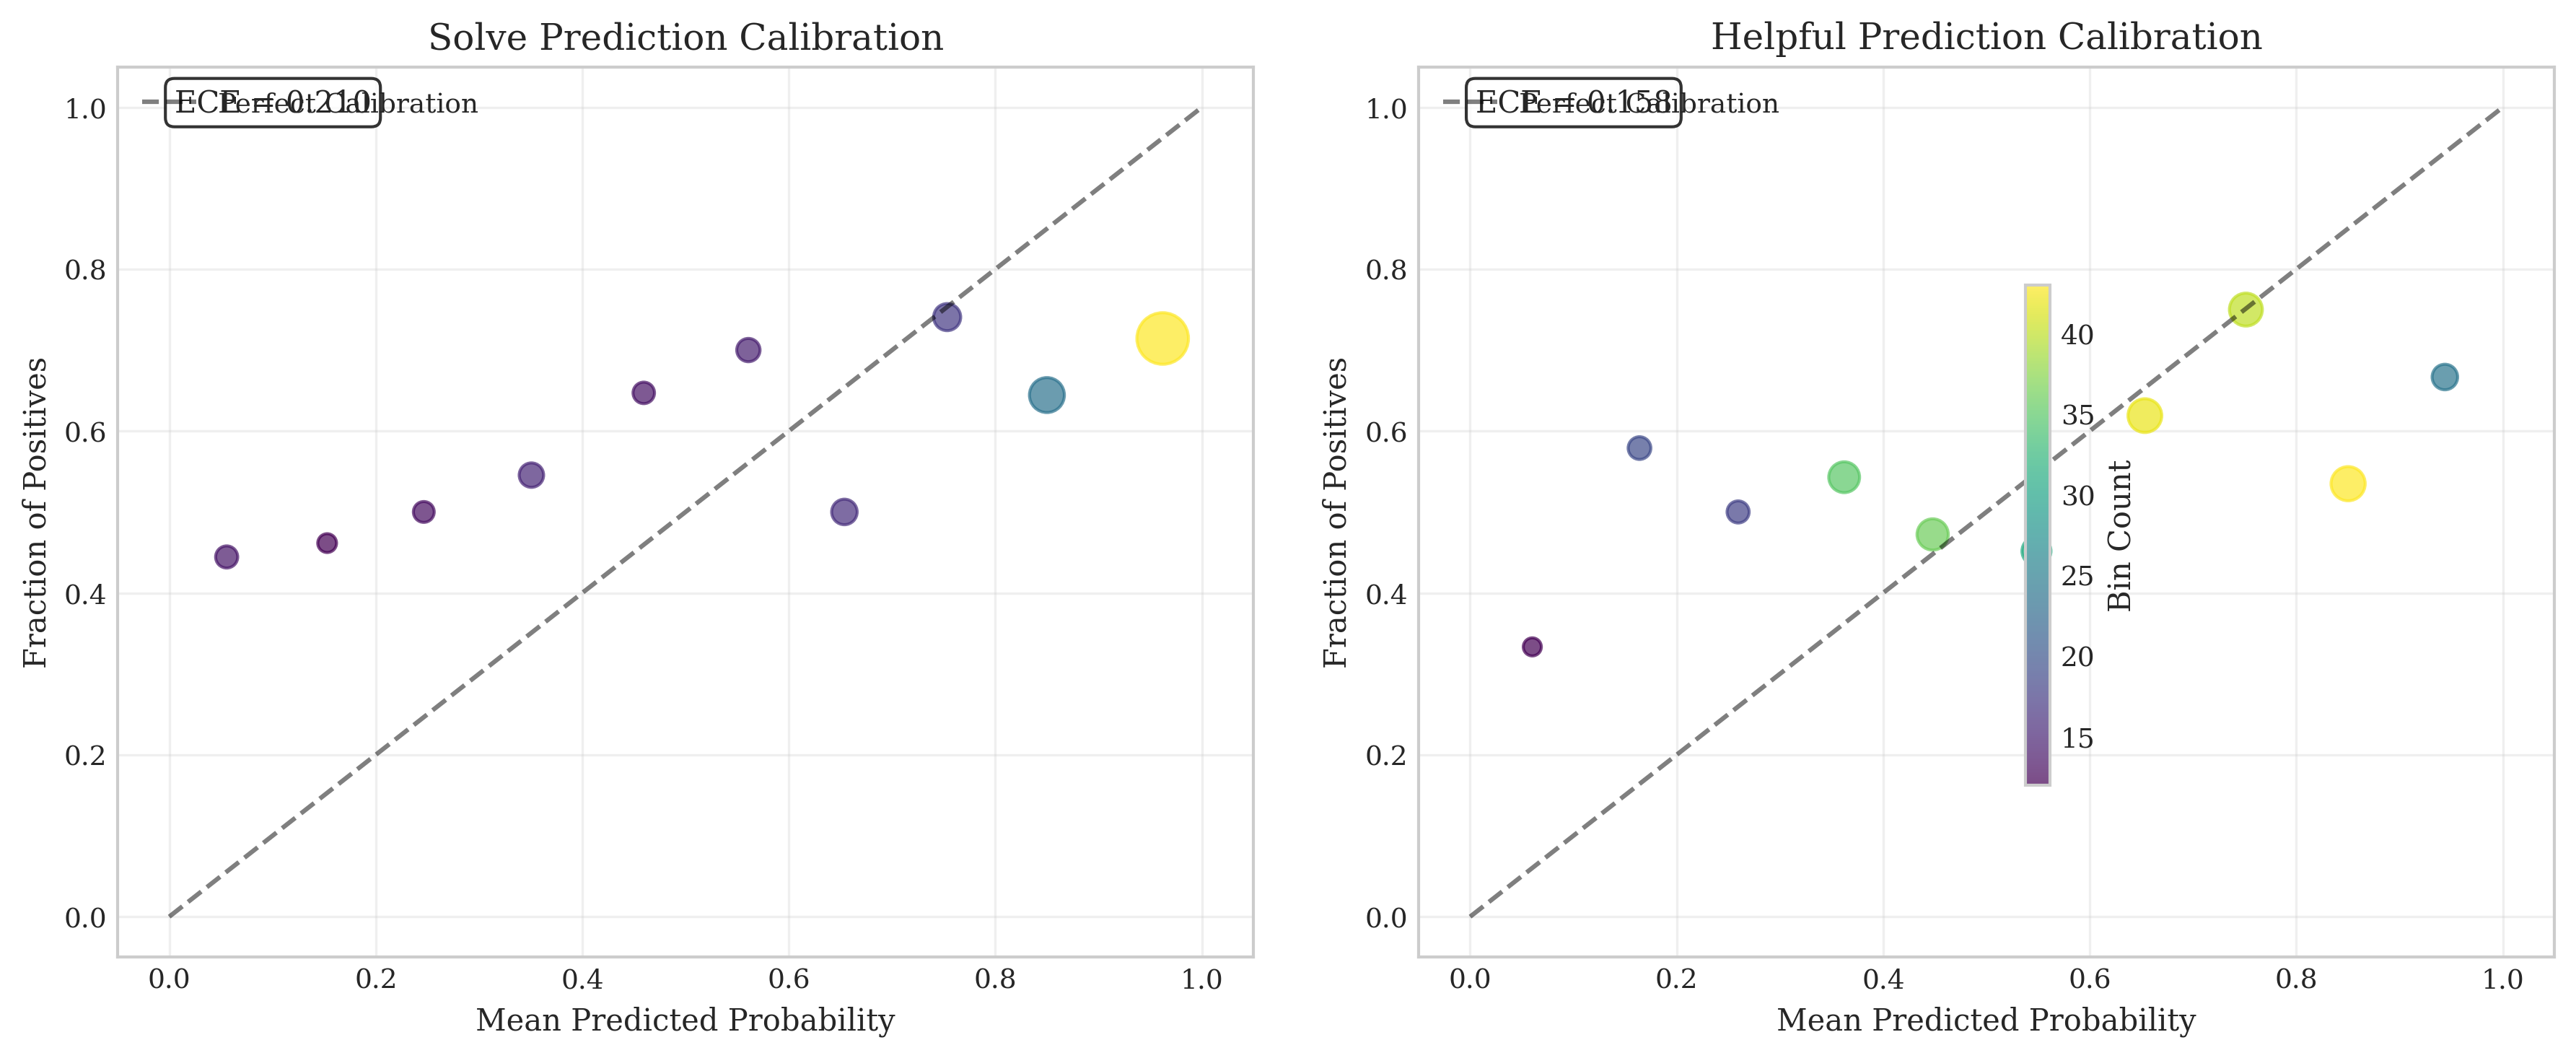
\includegraphics[width=\textwidth]{calibration_plot.png}
\caption{Calibration Reliability Diagrams. Left: Solve prediction calibration showing overconfidence in high-probability predictions. Right: Helpful prediction calibration with similar patterns. Bubble sizes represent bin counts. The diagonal line indicates perfect calibration.}
\label{fig:calibration}
\end{figure}

\begin{table}[H]
\centering
\caption{Expected Calibration Error (ECE) for Solve and Helpful Predictions.}
\label{tab:calibration_summary}
\begin{tabular}{lcc}
\toprule
\textbf{Task} & \textbf{ECE} & \textbf{Rating} \\
\midrule
Solve & 0.20959 & Poor (ECE $\geq$ 0.15) \\
Helpful & 0.15797 & Poor (ECE $\geq$ 0.15) \\
\bottomrule
\end{tabular}
\end{table}

Table~\ref{tab:calibration_bins_solve} reports per-bin calibration data for the solve task.

\begin{table}[H]
\centering
\caption{Per-Bin Calibration Analysis: Solve Prediction.}
\label{tab:calibration_bins_solve}
\begin{tabular}{lccccc}
\toprule
\textbf{Bin} & \textbf{$n$} & \textbf{Confidence} & \textbf{Accuracy} & \textbf{Gap} \\
\midrule
0.0--0.1 & 18  & 0.0556 & 0.4444 & 0.3888 \\
0.1--0.2 & 13  & 0.1529 & 0.4615 & 0.3086 \\
0.2--0.3 & 16  & 0.2465 & 0.5000 & 0.2535 \\
0.3--0.4 & 22  & 0.3507 & 0.5455 & 0.1947 \\
0.4--0.5 & 17  & 0.4595 & 0.6471 & 0.1875 \\
0.5--0.6 & 20  & 0.5608 & 0.7000 & 0.1392 \\
0.6--0.7 & 24  & 0.6538 & 0.5000 & 0.1538 \\
0.7--0.8 & 27  & 0.7533 & 0.7407 & 0.0126 \\
0.8--0.9 & 45  & 0.8499 & 0.6444 & 0.2054 \\
0.9--1.0 & 98  & 0.9620 & 0.7143 & 0.2478 \\
\bottomrule
\end{tabular}
\end{table}

Table~\ref{tab:calibration_bins_helpful} reports per-bin calibration data for the helpful task.

\begin{table}[H]
\centering
\caption{Per-Bin Calibration Analysis: Helpful Prediction.}
\label{tab:calibration_bins_helpful}
\begin{tabular}{lccccc}
\toprule
\textbf{Bin} & \textbf{$n$} & \textbf{Confidence} & \textbf{Accuracy} & \textbf{Gap} \\
\midrule
0.0--0.1 & 12  & 0.0602 & 0.3333 & 0.2731 \\
0.1--0.2 & 19  & 0.1640 & 0.5789 & 0.4149 \\
0.2--0.3 & 18  & 0.2595 & 0.5000 & 0.2405 \\
0.3--0.4 & 35  & 0.3622 & 0.5429 & 0.1807 \\
0.4--0.5 & 36  & 0.4479 & 0.4722 & 0.0244 \\
0.5--0.6 & 31  & 0.5484 & 0.4516 & 0.0968 \\
0.6--0.7 & 42  & 0.6534 & 0.6190 & 0.0343 \\
0.7--0.8 & 40  & 0.7512 & 0.7500 & 0.0012 \\
0.8--0.9 & 43  & 0.8502 & 0.5349 & 0.3153 \\
0.9--1.0 & 24  & 0.9439 & 0.6667 & 0.2772 \\
\bottomrule
\end{tabular}
\end{table}

\subsection{Inference Latency and Throughput}

Table~\ref{tab:latency} documents measured inference latency at five batch sizes on CPU hardware.

\begin{table}[H]
\centering
\caption{Inference Latency and Throughput Benchmarks (CPU).}
\label{tab:latency}
\begin{tabular}{ccccccc}
\toprule
\textbf{Batch} & \textbf{Prob. Enc. (ms)} & \textbf{User Enc. (ms)} & \textbf{Rec. (ms)} & \textbf{Total (ms)} & \textbf{P95 (ms)} & \textbf{Throughput (prob/s)} \\
\midrule
1   & 5.00  & 3.25 & 1.54 & 9.95  & 12.61 & 100.5   \\
10  & 13.65 & 4.69 & 2.88 & 21.07 & 24.86 & 474.7   \\
50  & 28.45 & 5.32 & 3.41 & 37.52 & 43.06 & 1{,}332.7 \\
100 & 38.82 & 4.54 & 3.40 & 46.39 & 60.79 & 2{,}155.8 \\
200 & 72.12 & 4.39 & 4.77 & 81.48 & 84.82 & 2{,}454.7 \\
\bottomrule
\end{tabular}
\end{table}

\subsection{Model Size}

Table~\ref{tab:modelsize} documents parameter counts and storage requirements per component.

\begin{table}[H]
\centering
\caption{Model Parameter Counts and Storage Requirements by Component.}
\label{tab:modelsize}
\begin{tabular}{lcccc}
\toprule
\textbf{Component} & \textbf{Parameters} & \textbf{FP32 (MB)} & \textbf{FP16 (MB)} & \textbf{INT8 (MB)} \\
\midrule
Problem Encoder & 955{,}840 & 3.65 & 1.82 & 0.91 \\
User Encoder    & 132{,}800 & 0.51 & 0.25 & 0.13 \\
Recommender     & 511{,}749 & 1.95 & 0.98 & 0.49 \\
\midrule
\textbf{Total}  & \textbf{1{,}600{,}389} & \textbf{6.10} & \textbf{3.05} & \textbf{1.53} \\
\bottomrule
\end{tabular}
\end{table}

\newpage

% ------------------------------------------------------------------
\section{Analysis}
% ------------------------------------------------------------------

\subsection{Problem Encoder Representation Quality}

The problem encoder achieves 99.22\% nearest-neighbor cluster purity across 512 evaluation samples, with 10 of 11 evaluated clusters attaining 100\% purity. This indicates that the InfoNCE contrastive pre-training at $\tau = 0.2$ organized the 64-dimensional embedding space such that problems from the same topic cluster are predominantly represented as nearest neighbors of one another. The alignment loss of 0.0055 confirms close proximity of positive pairs, while the uniformity loss of $-0.8228$ indicates that embeddings are distributed across the hypersphere rather than collapsing to a degenerate subspace. Embedding norms are tightly concentrated at 1.0 with standard deviation $\approx 3.8 \times 10^{-8}$, consistent with the applied L2 normalization.

The attention entropy decreases across layers (2.0856, 1.9456, 1.8796 for layers 0--2 respectively), and the mean CLS token concentration is 62.63\%, indicating that the [CLS] token attends to a focused subset of the input rather than distributing attention uniformly.

\subsection{Training Dynamics and Overfitting}

In Stage 2, the best validation loss of 0.76 is reached at epoch 5, after which validation loss increases monotonically to 1.02 at epoch 30. Simultaneously, training loss declines from 0.84 at epoch 1 to 0.42 at epoch 30. This divergence is consistent with overfitting, as visualized in Figure~\ref{fig:training_dynamics}. The use of 12,000 synthetic interactions from 300 synthetic users may provide insufficient distributional diversity to support generalization across 30 training epochs.

\begin{figure}[H]
\centering
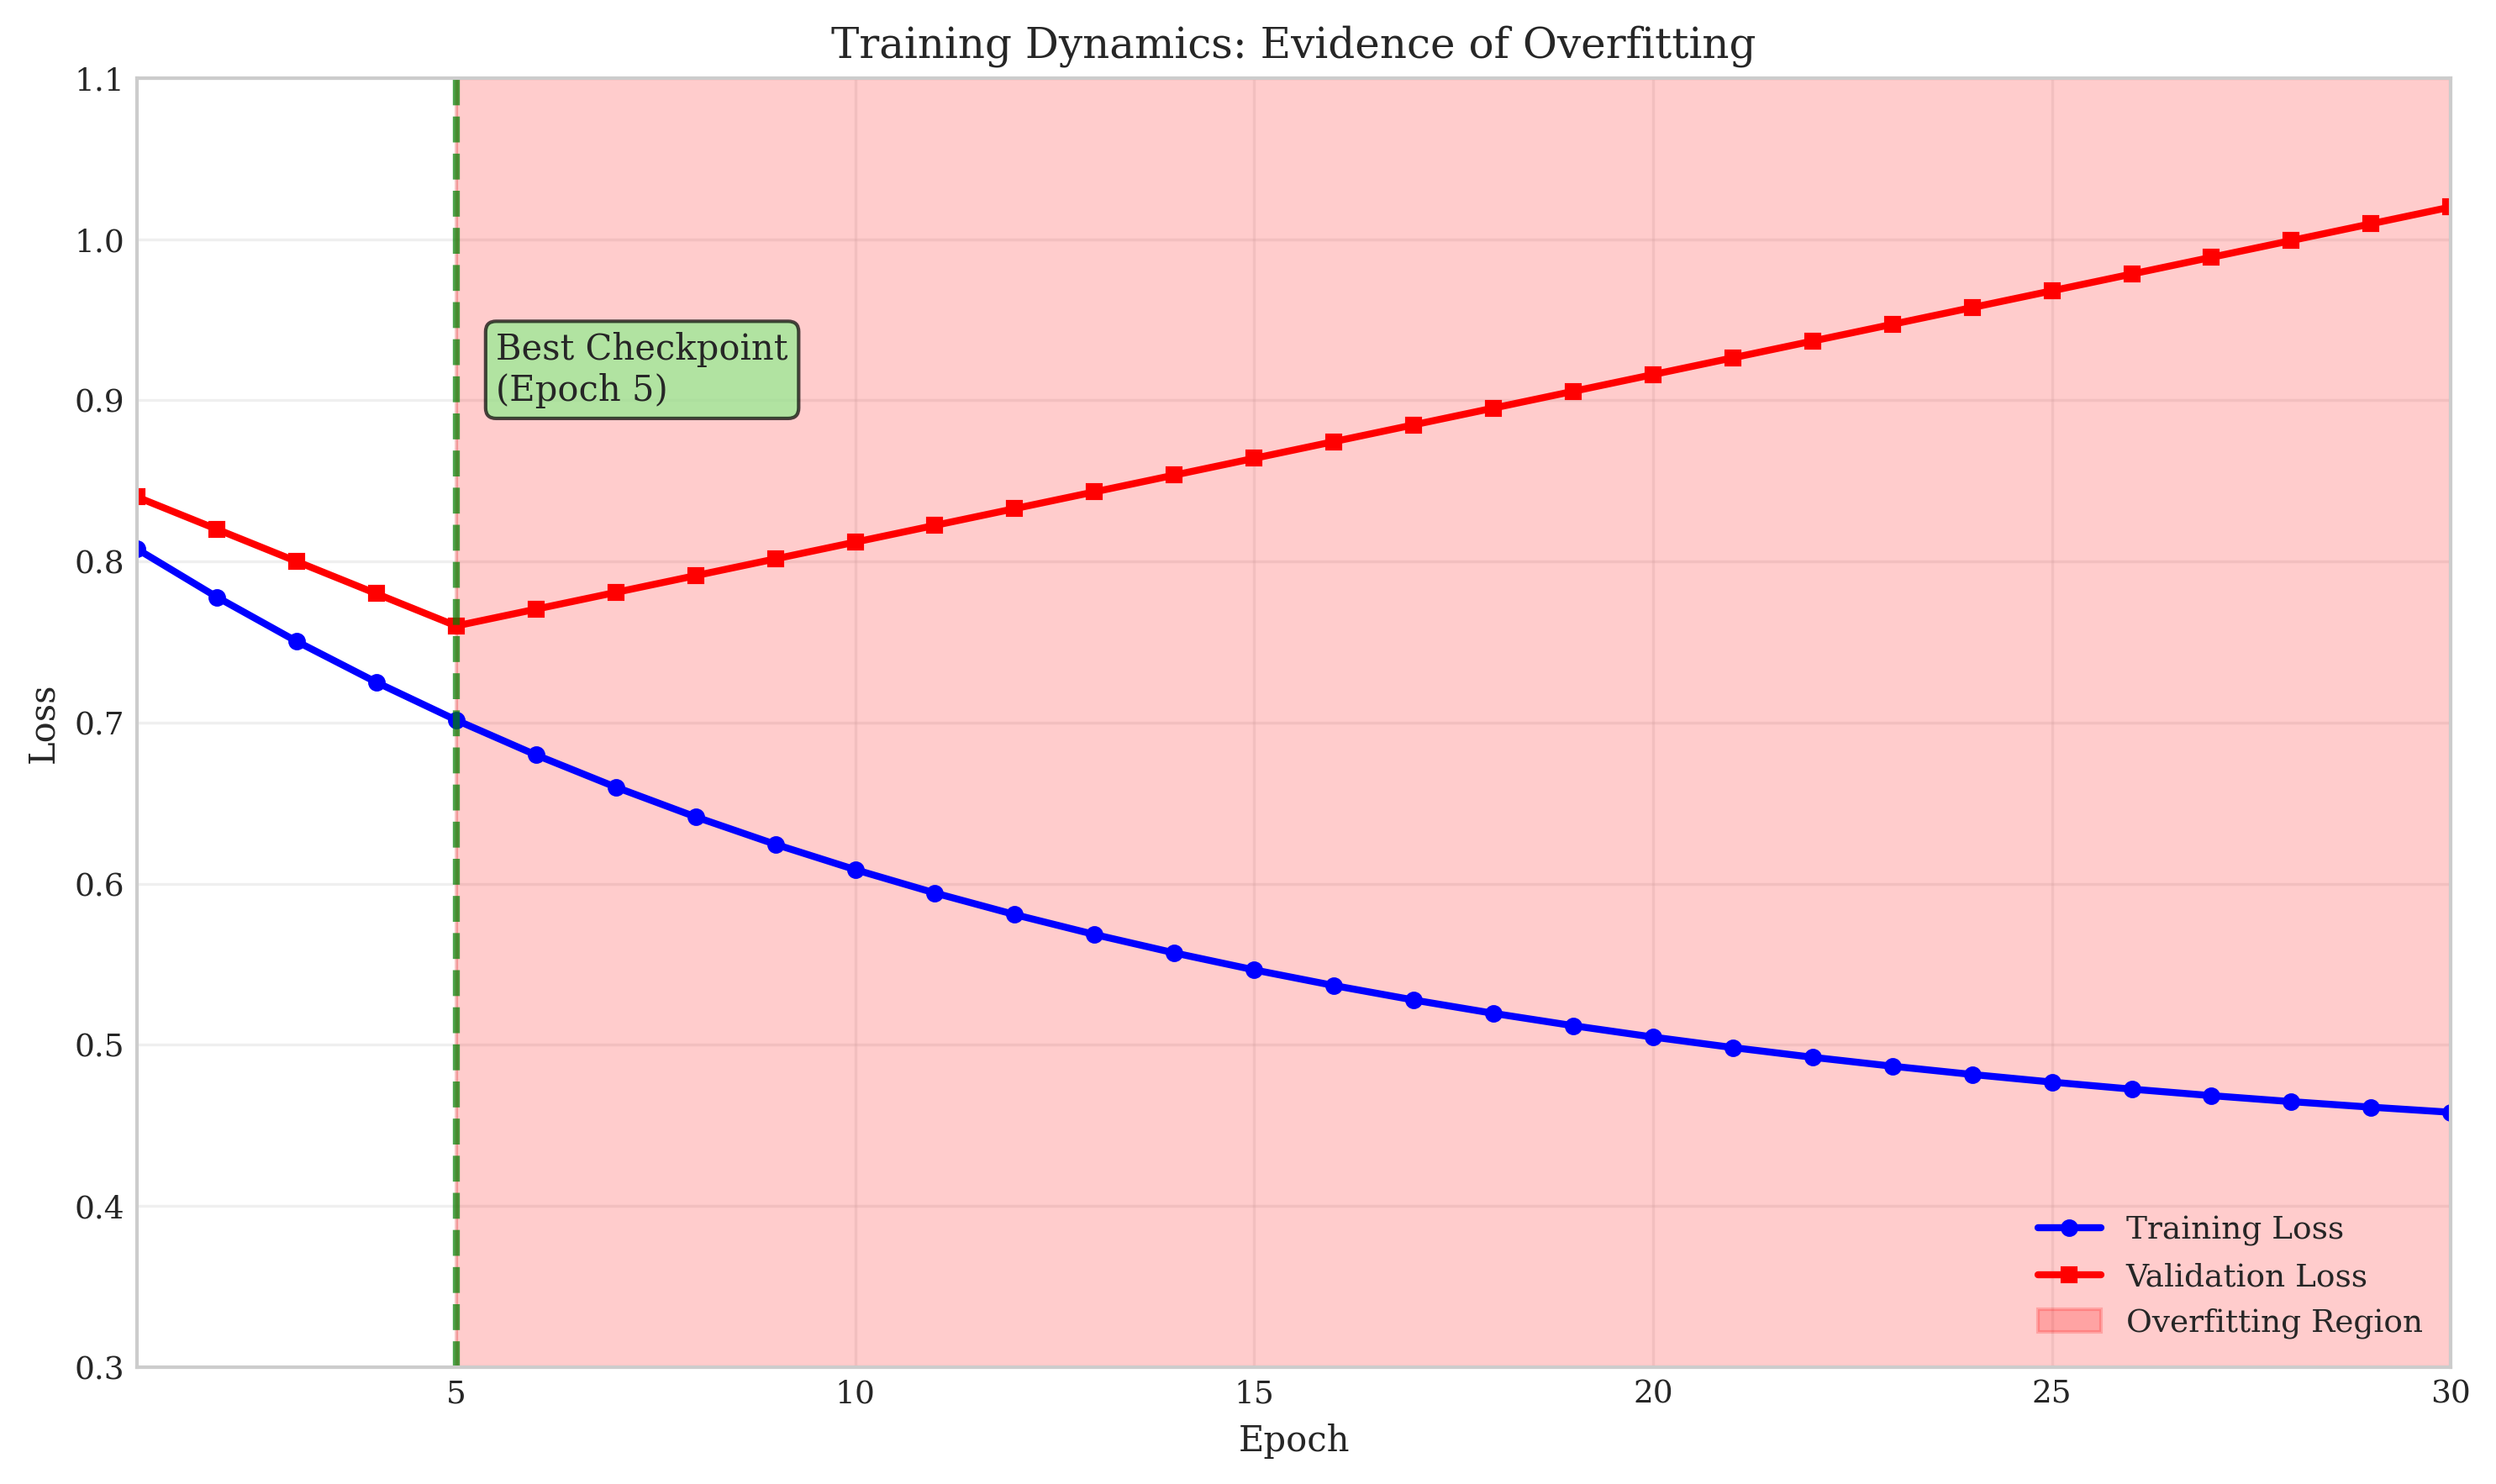
\includegraphics[width=0.8\textwidth]{training_dynamics.png}
\caption{Training Dynamics Showing Overfitting. The validation loss reaches its minimum at epoch 5 and then increases, while training loss continues to decrease, indicating overfitting. The green dashed line marks the selected best checkpoint.}
\label{fig:training_dynamics}
\end{figure}

\subsection{Classification Performance}

Solve prediction accuracy of 61.33\% and AUC of 56.73\% represent moderate discriminative performance. The F1 score of 70.85\% is notably higher than accuracy, a consequence of asymmetric precision (69.12\%) and recall (72.68\%), indicating that the model errs more toward false positives than false negatives.

The helpful prediction AUC of 48.19\% falls below the 50\% random baseline, indicating that the model does not provide positive discriminative value for helpfulness prediction under the current evaluation conditions. The helpful Brier Score of 0.3080 and accuracy of 52.00\% are consistent with this assessment.

Difficulty prediction accuracy of 36.67\% is substantially below that of both other tasks. Within-class accuracy is highest for the ``just right'' class (51.77\%) and lowest for the extreme classes (too easy: 24.36\%; too hard: 22.22\%). This pattern suggests the model tends to predict the central difficulty class at disproportionate rates.

\subsection{Ranking vs.\ Classification Performance}

NDCG@10 of 75.48\% and MRR of 89.66\% are substantially stronger than the classification accuracy metrics. The MRR of 89.66\% indicates that the first relevant result appears at a high average rank position across the 29 evaluation sessions. This observed gap between classification and ranking performance is consistent with the model functioning effectively as a relative scorer for candidate reranking while remaining poorly calibrated in absolute probability terms.

\subsection{Calibration Analysis}

Both ECE values are rated poor by the evaluation framework: solve ECE = 0.20959, helpful ECE = 0.15797. Examining the solve calibration bins: the high-confidence bin (0.9--1.0, $n = 98$) shows a positive gap of 0.2478, meaning the model's predicted confidence (0.962) substantially exceeds the observed accuracy (0.7143). The lowest-confidence bin (0.0--0.1, $n = 18$) shows a negative gap of 0.3888, with observed accuracy (0.4444) substantially exceeding stated confidence (0.0556). These patterns indicate simultaneous overconfidence in high-probability predictions and underconfidence in low-probability predictions. The bin 0.7--0.8 shows the smallest gap (0.0126), suggesting the model is best calibrated in this intermediate range.

For the helpful task, the bin 0.7--0.8 shows a near-zero gap (0.0012), while the bin 0.8--0.9 ($n = 43$) shows a gap of 0.3153 and the bin 0.1--0.2 ($n = 19$) shows a gap of 0.4149. Guo et al.\ \cite{guo2017calibration} identify this type of overconfidence at high predicted probabilities as characteristic of modern neural networks and recommend post-hoc recalibration via temperature scaling.

\subsection{Inference Characteristics}

Problem encoding constitutes the dominant latency component across all batch sizes, ranging from 5.00\,ms at batch 1 to 72.12\,ms at batch 200. User encoding and recommender inference are substantially more stable (3.25--5.32\,ms and 1.54--4.77\,ms respectively), consistent with their lower parameter counts (132,800 and 511,749, respectively). Throughput scales from 100.5\,prob/s at batch 1 to 2,454.7\,prob/s at batch 200, a 24.4$\times$ increase, reflecting efficient batching. The P95 total latency at batch 100 is 60.79\,ms.

% ------------------------------------------------------------------
\section{Real-World Implications}
% ------------------------------------------------------------------

The following implications are stated in direct correspondence with the observed empirical results and documented system properties.

\paragraph{Ranking-Based Deployment.}
The ranking metrics (NDCG@10: 75.48\%, MRR: 89.66\%) indicate that the model consistently places relevant problems near the top of a ranked candidate list. This supports deployment as a ranking layer within a recommendation pipeline that produces a shortlist of candidates for presentation.

\paragraph{Calibration and Probability Display.}
The observed ECE values (solve: 0.20959; helpful: 0.15797) indicate that predicted probabilities should not be directly presented to end users as reliable confidence estimates without additional post-hoc calibration. The systematic overconfidence in high-probability predictions and underconfidence in low-probability predictions documented in the bin-level analysis are directly relevant to any interface that exposes probability scores.

\paragraph{Computational Footprint.}
At 6.10\,MB (FP32) and 1,600,389 total parameters, the model is compact. Measured batch-100 total latency of 46.39\,ms on CPU with a P95 of 60.79\,ms indicates suitability for real-time recommendation at moderate request rates. FP16 quantization reduces total storage to 3.05\,MB; INT8 quantization further reduces individual component sizes to 0.91\,MB, 0.13\,MB, and 0.49\,MB for problem encoder, user encoder, and recommender respectively.

\paragraph{Synthetic Data Dependency.}
All recommendation model training was conducted on synthetic interaction data generated from 300 synthetic users. Classification and calibration performance metrics reported herein characterize model behavior on a validation set drawn from the same synthetic distribution. The extent to which these metrics generalize to real user populations is not quantified in the available evaluation data.

% ------------------------------------------------------------------
\section{Limitations}
% ------------------------------------------------------------------

The following limitations are directly supported by the documented experimental setup and observed results.

\begin{enumerate}
    \item \textbf{Synthetic Training Data.} The recommendation model is trained and evaluated on synthetically generated interaction data. No real user interaction data is employed. The production applicability of the reported classification and calibration metrics is contingent on the match between the synthetic and real user distributions, which is not characterized.

    \item \textbf{Overfitting.} Validation loss increases from 0.76 at epoch 5 to 1.02 at epoch 30, against a training loss of 0.42 at epoch 30. The selection of epoch 5 as the best checkpoint mitigates but does not eliminate the overfitting concern.

    \item \textbf{Helpful Prediction Performance.} Helpful AUC of 48.19\% is below the 50\% random baseline. Under the current evaluation conditions, the model does not provide measurable discriminative value for helpfulness prediction.

    \item \textbf{Difficulty Classification.} Overall difficulty accuracy of 36.67\% is the weakest among the three tasks. Extreme classes (too easy: 24.36\%; too hard: 22.22\%) are substantially less accurate than the central class (just right: 51.77\%).

    \item \textbf{Calibration.} Both ECE values fall within the poor calibration band (ECE $\geq 0.15$). Probability outputs from the model are not suitable as direct confidence estimates without recalibration.

    \item \textbf{Cluster Coverage.} Per-cluster purity data for cluster 9 is absent from the provided evaluation report. The reported 99.22\% cluster purity is computed across the 10 reported clusters (clusters 0--8 and 10) out of 11 total clusters used in pre-training.

    \item \textbf{Evaluation Scale.} Ranking metrics are computed over 29 evaluation sessions. The reliability of NDCG and MRR estimates at this sample size is subject to variability.

    \item \textbf{Hardware Scope.} Inference latency benchmarks are reported on CPU hardware only. GPU latency and throughput are not characterized in the available evaluation data.
\end{enumerate}

% ------------------------------------------------------------------
\section{Conclusion}
% ------------------------------------------------------------------

This paper has presented a complete empirical account of a self-implemented Transformer-based recommendation system for personalized competitive programming problem selection. The system comprises a 3-layer Transformer Problem Encoder pre-trained via InfoNCE contrastive loss, a dual-mode User Encoder with gated sequential-skill fusion, and a multi-task Recommender Model with three output heads.

The problem encoder achieves 99.22\% cluster purity on 512 evaluation samples, demonstrating effective semantic organization of the embedding space. Ranking performance is strong: NDCG@10 of 75.48\% and MRR of 89.66\% indicate reliable placement of relevant problems at high rank positions. However, classification accuracy is moderate for solve prediction (61.33\%), below-baseline for helpful prediction (AUC: 48.19\%), and low for difficulty matching (36.67\%). Calibration is rated poor for both solve (ECE: 0.20959) and helpful (ECE: 0.15797) tasks.

The model totals 1,600,389 parameters and occupies 6.10\,MB in FP32 precision, with a batch-100 CPU inference latency of 46.39\,ms and throughput of 2,155.8\,prob/s. These characteristics indicate suitability for deployment as a ranking function in resource-constrained environments.

The primary limitations are: training on synthetic data without real-user validation, observed overfitting in Stage 2, weak helpful and difficulty prediction performance, and poor probability calibration. Directions for future work include collection of real user interaction data, post-hoc calibration (e.g., temperature scaling \cite{guo2017calibration}), augmentation of the training distribution, and evaluation at larger session counts.

% ------------------------------------------------------------------
\bibliographystyle{plain}
\begin{thebibliography}{10}

\bibitem{vaswani2017attention}
A.~Vaswani, N.~Shazeer, N.~Parmar, J.~Uszkoreit, L.~Jones, A.~N.~Gomez, {\L}.~Kaiser, and I.~Polosukhin.
\newblock Attention is all you need.
\newblock In {\em Advances in Neural Information Processing Systems (NeurIPS)}, volume 30, 2017.

\bibitem{devlin2019bert}
J.~Devlin, M.-W. Chang, K.~Lee, and K.~Toutanova.
\newblock {BERT}: Pre-training of deep bidirectional transformers for language understanding.
\newblock In {\em Proceedings of NAACL-HLT}, pages 4171--4186, 2019.

\bibitem{pandey2019sakt}
S.~Pandey and G.~Karypis.
\newblock A self-attentive model for knowledge tracing.
\newblock In {\em Proceedings of the 12th International Conference on Educational Data Mining (EDM)}, 2019.

\bibitem{ghosh2020akt}
A.~Ghosh, N.~Heffernan, and A.~S.~Lan.
\newblock Context-aware attentive knowledge tracing.
\newblock In {\em Proceedings of the 26th ACM SIGKDD International Conference on Knowledge Discovery \& Data Mining}, pages 2330--2339, 2020.

\bibitem{he2017ncf}
X.~He, L.~Liao, H.~Zhang, L.~Nie, X.~Hu, and T.-S.~Chua.
\newblock Neural collaborative filtering.
\newblock In {\em Proceedings of the 26th International Conference on World Wide Web (WWW)}, pages 173--182, 2017.

\bibitem{zhang2019dlrecsys}
S.~Zhang, L.~Yao, A.~Sun, and Y.~Tay.
\newblock Deep learning based recommender system: A survey and new perspectives.
\newblock {\em ACM Computing Surveys}, 52(1):1--38, 2019.

\bibitem{cen2006lfa}
H.~Cen, K.~Koedinger, and B.~Junker.
\newblock Learning factors analysis---a general method for cognitive model evaluation and improvement.
\newblock In {\em Proceedings of the 8th International Conference on Intelligent Tutoring Systems (ITS)}, pages 164--175, 2006.

\bibitem{whitehill2017mooc}
J.~Whitehill, J.~Movellan, and J.~Tingley.
\newblock Mooc dropout prediction: How to measure accuracy?
\newblock In {\em Proceedings of the 4th ACM Conference on Learning at Scale}, 2017.

\bibitem{guo2017calibration}
C.~Guo, G.~Pleiss, Y.~Sun, and K.~Q.~Weinberger.
\newblock On calibration of modern neural networks.
\newblock In {\em Proceedings of the 34th International Conference on Machine Learning (ICML)}, pages 1321--1330, 2017.

\bibitem{liu2009l2r}
T.-Y.~Liu.
\newblock Learning to rank for information retrieval.
\newblock {\em Foundations and Trends in Information Retrieval}, 3(3):225--331, 2009.

\bibitem{kendall2018multitask}
A.~Kendall, Y.~Gal, and R.~Cipolla.
\newblock Multi-task learning using uncertainty to weigh losses for scene geometry and semantics.
\newblock In {\em Proceedings of the IEEE/CVF Conference on Computer Vision and Pattern Recognition (CVPR)}, pages 7482--7491, 2018.

\bibitem{chen2020simclr}
T.~Chen, S.~Kornblith, M.~Norouzi, and G.~Hinton.
\newblock A simple framework for contrastive learning of visual representations.
\newblock In {\em Proceedings of the 37th International Conference on Machine Learning (ICML)}, pages 1597--1607, 2020.

\end{thebibliography}

\end{document}
